\documentclass[runningheads]{llncs}

\usepackage{graphicx}
\usepackage{amsmath,amssymb}
\usepackage{booktabs}
\usepackage{hyperref}
\usepackage{tikz}
\usetikzlibrary{positioning,arrows.meta,calc}

\newcommand{\sayan}[1]{\textcolor{blue}{[Sayan: #1]}}

\begin{document}

\title{Abstract Rendering Toolkit for}
\author{Author Name}
\institute{Your Institution}

\maketitle

\begin{abstract}
    \sayan{Write later.}
\end{abstract}

\section{Introduction}
\label{sec:introduction}

Abstract rendering~\cite{AbstractRendering_Neurips2025} is a recently developed technique for over-approximating the set of all possible rendered images that can result from a set of camera poses and 3D scenes with semantic uncertainties. In a nutshell, abstract rendering takes as input a bounded set of camera poses---defined by interval pose matrices---and a set of scenes represented by 3D Gaussian spats (3DGS)~\cite{3DGS}, and propagates these sets through the standard 3DGS rendering algorithm to compute the output set of {\em abstract images}, which are represented by per-pixel color intervals or linear bounds. The key enabler for this technique is a set of piecewise linear relational abstractions for certain primitive nonlinear operations (such as ...) that appear in the rendering algorithm and careful engineering of the composition of these abstractions in the Crown~\cite{zhang2018efficient} bound propagation framework to ensure tightness of the final abstract images.

Previous work has demonstrated the feasibility  of abstract rendering in certifying the robustness of image processing models like classifiers and object detectors against {\em small ranges\/} of semantic purterbations, such as planar camera movements around a target object  and lighting changes. For larger-scale applications, such as verifying vision-based controllers operating in large scenes, abstract rendering needs to be integrated into a larger verification workflow that can efficiently specify, partition, and manage the large number of abstract rendering queries that arise in such settings.

This paper introduces an open-source toolkit for abstract rendering to the verification community. Our toolkit provides a user-friendly interface for defining 3D scenes with semantic uncertainties, specifying camera parameters, 
\sayan{Highlights, results, technical challenges.}

\section{Using the Abstract Rendering Toolkit}
\label{sec:art}

\paragraph{Running example and workflow.}
We use the task of verifying a vision-based pose estimator, GateNet~\cite{}, over a large pose space in a drone racing arena as a running example in this paper.


\begin{figure}[ht]
    \centering
    \resizebox{\linewidth}{!}{%
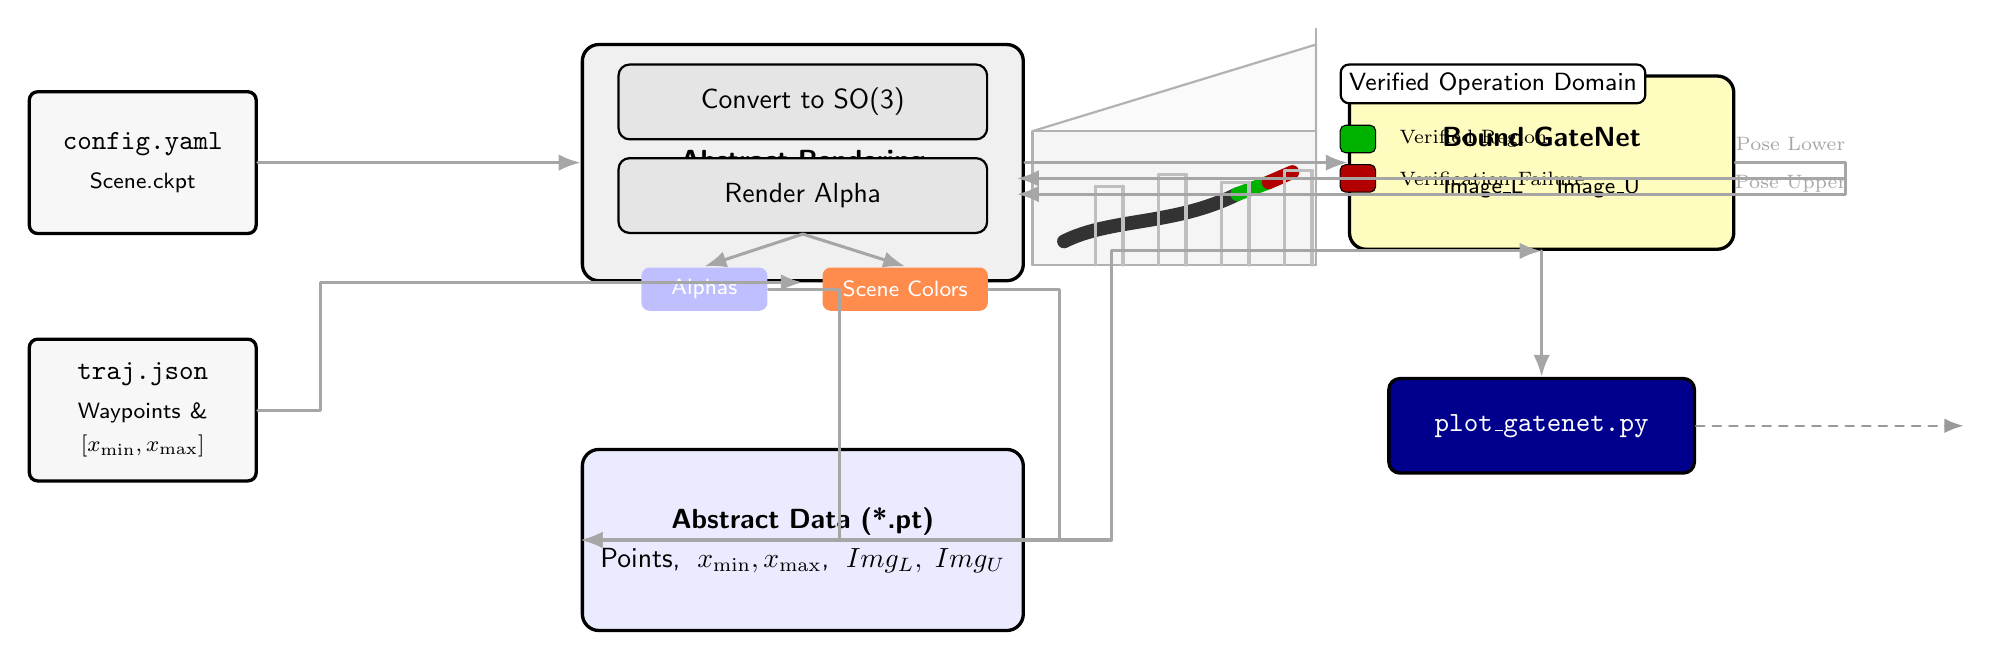
\begin{tikzpicture}[
    font=\sffamily,
    line join=round,
    line cap=round,
    >=Latex,
    node distance=1.4cm and 3.8cm,
    every node/.style={inner sep=4pt},
    filebox/.style={draw, rounded corners=3pt, fill=gray!6, very thick,
        minimum width=2.7cm, minimum height=1.8cm, text width=2.6cm, align=center},
    proc/.style={draw, rounded corners=6pt, fill=gray!12, very thick,
        minimum width=5.6cm, minimum height=3.0cm, text width=5.2cm, align=center},
    subproc/.style={draw, rounded corners=4pt, fill=gray!20, thick,
        minimum width=4.6cm, minimum height=0.95cm, text width=4.4cm, align=center},
    data/.style={draw, rounded corners=6pt, fill=blue!8, very thick,
        minimum width=5.6cm, minimum height=2.3cm, text width=5.2cm, align=center},
    model/.style={draw, rounded corners=6pt, fill=yellow!25, very thick,
        minimum width=4.8cm, minimum height=2.2cm, text width=4.6cm, align=center},
    script/.style={draw, rounded corners=4pt, fill=blue!55!black, text=white, very thick,
        minimum width=3.8cm, minimum height=1.2cm, text width=3.6cm, align=center},
    legendbox/.style={draw, rounded corners=2pt, minimum width=0.45cm, minimum height=0.35cm},
    callout/.style={draw, fill=white, rounded corners=3pt, thick, inner sep=3pt},
    dashedflow/.style={dash pattern=on 3pt off 3pt, line width=0.9pt, gray!80},
    flow/.style={-Latex, line width=1.1pt, gray!70}
]

% Inputs
\node[filebox] (config) {\texttt{config.yaml}\\[2pt]\footnotesize Scene.ckpt};
\node[filebox, below=1.3cm of config] (traj) {\texttt{traj.json}\\[2pt]\footnotesize Waypoints \& $[x_{\min},x_{\max}]$};

% Abstract rendering block
\node[proc, right=4.1cm of config] (render) {\textbf{Abstract Rendering}};
  % substeps inside rendering
  \node[subproc] (so3) at ($(render.north)+(0,-0.75)$) {Convert to SO(3)};
  \node[subproc] (alpha) at ($(so3.south)+(0,-0.7)$) {Render Alpha};
  \node[rounded corners=3pt, fill=blue!25, text=white, thick, minimum width=1.6cm, minimum height=0.55cm]
        (alphas) at ($(alpha.south)+(-1.25,-0.7)$) {\footnotesize Alphas};
  \node[rounded corners=3pt, fill=red!30!orange!70, text=white, thick, minimum width=2.1cm, minimum height=0.55cm]
        (colors) at ($(alpha.south)+(1.3,-0.7)$) {\footnotesize Scene Colors};

% Abstract data
\node[data, below=2.1cm of render] (adata) {\textbf{Abstract Data (*.pt)}\\[2pt]
Points,\; $x_{\min}, x_{\max}$,\; $Img_L,\; Img_U$};

% Bound GateNet
\node[model, right=4.1cm of render] (gatenet) {\textbf{Bound GateNet}\\[4pt]
\begin{tabular}{cc}
\footnotesize Image\_L & \footnotesize Image\_U\\[-2pt]
\end{tabular}};

% plot_gatenet
\node[script, below=1.6cm of gatenet] (plot) {\texttt{plot\_gatenet.py}};

% 3D verified plot (stylized)
\begin{scope}[shift={(11.3, -1.3)}]
  \coordinate (plotOrigin) at (0,0);
  \draw[fill=gray!4, draw=gray!60, thick] (0,0) -- (3.6,1.1) -- (3.6,2.8) -- (0,1.7) -- cycle; % top
  \draw[fill=gray!8, draw=gray!60, thick] (0,0) rectangle (3.6,1.7); % floor
  \draw[fill=gray!10, draw=gray!60, thick] (3.6,0) -- (3.6,1.7) -- (3.6,3.0) -- (3.6,1.1) -- cycle; % side
  % tube path
  \draw[line width=5pt, draw=black!80] (0.4,0.3) .. controls (1.0,0.6) and (1.8,0.5) .. (2.6,0.9);
  \draw[line width=5pt, draw=green!70!black] (2.6,0.9) -- (3.0,1.05);
  \draw[line width=5pt, draw=red!70!black] (3.0,1.05) -- (3.3,1.18);
  % gates
  \foreach \x/\h in {0.8/1.0,1.6/1.15,2.4/1.05,3.2/1.2}{
    \draw[gray!50, line width=1.2pt] (\x,0) -- (\x,\h);
    \draw[gray!50, line width=1.2pt] (\x+0.35,0) -- (\x+0.35,\h);
    \draw[gray!50, line width=1.2pt] (\x, \h) -- (\x+0.35,\h);
  }
  % legend
  \node[callout, anchor=west, align=left] at (3.9,2.3) {\small Verified Operation Domain};
  \node[legendbox, fill=green!70!black, anchor=west] (leg1) at (3.9,1.6) {};
  \node[anchor=west, font=\scriptsize] at ($(leg1.east)+(0.15,0)$) {Verified Region};
  \node[legendbox, fill=red!70!black, anchor=west] (leg2) at (3.9,1.1) {};
  \node[anchor=west, font=\scriptsize] at ($(leg2.east)+(0.15,0)$) {Verification Failure};
\end{scope}

% Flow arrows
\draw[flow] (config.east) -- ++(0.8,0) |- (render.west);
\draw[flow] (traj.east) -- ++(0.8,0) |- (render.south);
\draw[flow] (alpha.south) -- (alphas.north);
\draw[flow] (alpha.south) -- (colors.north);
\draw[flow] (alphas.east) -- ++(0.9,0) |- (adata.west);
\draw[flow] (colors.east) -- ++(0.9,0) |- (adata.west);
\draw[flow] (render.east) -- (gatenet.west);
\draw[flow] (adata.east) -- ++(1.1,0) |- (gatenet.south);
\draw[flow] (gatenet.east) -- ++(1.4,0) node[midway, above, font=\scriptsize] {Pose Lower} |- (11.1, -0.2);
\draw[flow] (gatenet.east) -- ++(1.4,0) node[midway, below, font=\scriptsize] {Pose Upper} |- (11.1, -0.4);
\draw[flow] (gatenet.south) -- (plot.north);
\draw[dashedflow, -Latex] (plot.east) -- ++(3.4,0);

\end{tikzpicture}%
}%

    \caption{Abstract rendering workflow from inputs to GateNet verification output.}
    \label{fig:art-workflow}
\end{figure}

There are several steps and user-interfaces involved in performing such a large-scale verification task: (1) the user has to specify the input pose and scene spaces, (2) these spaces have to be then partitioned into smaller cells according to user-defined parameters, (3)  the abstract rendering engine is then run on these cells and the resulting abstract images are stored in a dictionary, (4) each abstract image from the dictionary is  passed through GateNet using a bound propagation tool like Crown~\cite{} to verify whether the pose estimator is robust over that cell, and (5) finally the verification results are collected for analysis and visualization. Figure~\ref{fig:art-workflow} illustrates this workflow. In the following paragraphs, we describe the modules of the toolkit that support each of these steps.

\paragraph{Input pose and scene spaces.}
\sayan{Fill in details; try to be precise, use math where it makes sens, e.g., pose space is a subset of SE(3), etc., but dont go overboard.}


A planner yields a nominal trajectory $\gamma:[0,T]\to\mathbb{R}^3$ as waypoints $(p_i)$ with a smooth camera orientation field $R:[0,T]\to SO(3)$. Operational uncertainty is a tube
\[
\mathcal{P} = \{(p,R(t)) \mid p \in B(p(t),\Delta_t),\, t\in[0,T]\} \subset SE(3),
\]
where $\Delta_t$ encodes tracking error budgets. This bounded subset of $SE(3)$ is the pose space given to the toolkit.

\paragraph{1) Pose standard and validation.}
Poses are represented as homogeneous transforms $\begin{bmatrix}R&p\\0&1\end{bmatrix}$ with per-waypoint translation tubes $B(p_i,\Delta_i)$ and optional attitude jitter. The validator rejects non-orthogonal $R$, clamps drift, and ensures tube continuity, so downstream bounds remain well-conditioned.

\paragraph{2) Partitioning interface.}
The pose/scene tube is split into solver-ready regions. Splits are anisotropic: finer near gates or high-curvature segments, coarser on straights. Users pick a budget (\verb|--cells 200|) or tolerance (e.g., $0.15$\,m / $2^\circ$); the tool refines only where image Jacobians w.r.t. pose exceed a threshold, keeping AR tight without exploding cell count.

\paragraph{3) AR results dictionary.}
For each region the AR engine stores alpha bounds, color bounds, and lower/upper images keyed by (pose cell, scene cell, AR config, model hash). This cache avoids rerunning heavy rendering and supports instant plotting (\verb|ar plot --cell 42|) to visualize appearance variability near a gate.

\paragraph{4) Verification dictionary and downstream use.}
GateNet (or any consumer) reads the cached envelopes and records per-cell outcomes: verified / failed / unknown. Keys align with the AR dictionary, so failures trace back to their pose tube and gate. Verdicts can be overlaid on the trajectory via \verb|plot_gatenet.py|, yielding a green (verified) / red (failed) lap-level map.

\paragraph{Workflow.}
\begin{enumerate}
    \item \verb|pose validate traj.json --tube 0.2| builds the $SE(3)$ tube.
    \item \verb|pose partition --budget 180| generates focused cells near gates.
    \item \verb|ar run --cells all| populates the AR dictionary.
    \item \verb|verify gatenet --cells all| emits robustness verdicts.
    \item \verb|plot_gatenet.py| visualizes per-cell results along the flight path.
\end{enumerate}

\paragraph{Technical highlights.}
Conditioning of $R$ is preserved during interpolation, avoiding $\det R\neq 1$ drift; anisotropic partitioning targets pose directions with high image sensitivity; cached envelopes are compressed without widening bounds; per-cell verdicts compose to a lap-level statement while accounting for overlapping tubes.



\section{Experimental Results}
\label{sec:experiments}

We evaluate the Abstract Rendering Toolkit (ART) on verifying the robustness of a pretrained GateNet-based pose estimator in $4$ different drone racing tracks created in a 3DGS environment built using FalconGym~\cite{falcon}. The four tracks correspond to $4$ racing gates placed in a flying arena in different layouts: (1) a straight track, (2) a circular track, (3) a lemminiscate track, and (4) ??. 

\sayan{Describe the different inputs at an appropriate level of detail. Not all numbers need to be spelled out.}

\sayan{Show qualitative results with the 3Dplots}

\sayan{Main takeaways. What are they and how do you justify them?}

\section{Conclusion}
\label{sec:conclusion}
\sayan{Write later.}



\bibliographystyle{splncs04}
\bibliography{egbib}

\end{document}
